\documentclass[red]{tutorial}
\usepackage[no-math]{fontspec}
\usepackage{xpatch}
	\renewcommand{\ttdefault}{ul9}
	\xpatchcmd{\ttfamily}{\selectfont}{\fontencoding{T1}\selectfont}{}{}
	\DeclareTextCommand{\nobreakspace}{T1}{\leavevmode\nobreak\ }
\usepackage{polyglossia} % English please
	\setdefaultlanguage[variant=us]{english}
%\usepackage[charter,cal=cmcal]{mathdesign} %different font
%\usepackage{avant}
\usepackage{microtype} % Less badboxes


\usepackage[charter,cal=cmcal]{mathdesign} %different font
%\usepackage{euler}
 
\usepackage{blindtext}
\usepackage{calc, ifthen, xparse, xspace}
\usepackage{makeidx}
\usepackage[hidelinks, urlcolor=blue]{hyperref}   % Internal hyperlinks
\usepackage{mathtools} % replaces amsmath
\usepackage{bbm} %lower case blackboard font
\usepackage{amsthm, bm}
\usepackage{thmtools} % be able to repeat a theorem
\usepackage{thm-restate}
\usepackage{graphicx}
\usepackage{xcolor}
\usepackage{multicol}
\usepackage{fnpct} % fancy footnote spacing

 
\newcommand{\xh}{{{\mathbf e}_1}}
\newcommand{\yh}{{{\mathbf e}_2}}
\newcommand{\zh}{{{\mathbf e}_3}}
\newcommand{\R}{\mathbb{R}}
\newcommand{\Z}{\mathbb{Z}}
\newcommand{\N}{\mathbb{N}}
\newcommand{\proj}{\mathrm{proj}}
\newcommand{\Proj}{\mathrm{proj}}
\newcommand{\Perp}{\mathrm{perp}}
\renewcommand{\span}{\mathrm{span}\,}
\newcommand{\Span}{\mathrm{span}\,}
\newcommand{\Img}{\mathrm{img}\,}
\newcommand{\Null}{\mathrm{null}\,}
\newcommand{\Range}{\mathrm{range}\,}
\newcommand{\rref}{\mathrm{rref}}
\newcommand{\rank}{\mathrm{rank}}
\newcommand{\Rank}{\mathrm{rank}}
\newcommand{\nnul}{\mathrm{nullity}}
\newcommand{\mat}[1]{\begin{bmatrix}#1\end{bmatrix}}
\newcommand{\chr}{\mathrm{char}}
\renewcommand{\d}{\mathrm{d}}


\theoremstyle{definition}
\newtheorem{example}{Example}[section]
\newtheorem{defn}{Definition}[section]

%\theoremstyle{theorem}
\newtheorem{thm}{Theorem}[section]

\pgfkeys{/tutorial,
	name={Tutorial 1},
	author={Jason Siefken \& Bernardo Galv\~ao-Sousa},
	course={MAT 244},
	date={},
	term={},
	title={Limits of Numerics}
	}

\begin{document}
	\begin{tutorial}
				\begin{objectives}
			In this tutorial, you will explore applications of Euler's method for approximating solutions to ODEs
			and the limits of Euler's method.

			These problems relate to the following course learning
			objective: \textit{work independently to understand concepts and procedures that have not
			been previously explained to you}.
		\end{objectives}

	%	\bigskip


		\subsection*{Problems}
		
		Consider the differential equations
		\begin{equation}
			\label{tut1-ode}
			y'=\frac{4\sin(4x)}{1+y}
		\end{equation}
		\begin{equation}
			\label{tut1-ode2}
			y'=4\sin(4x)
		\end{equation}

		\begin{enumerate}
			\item Create a spread sheet that can approximate solutions to Equation \eqref{tut1-ode} with initial condition $y(0)=0$. Make sure you
			can adjust the step size (i.e., $\Delta$) in your spread sheet.
				\begin{enumerate}
					\item Justify both with a simulation and analytically (i.e. from the equation) whether or not $y(x)=0$
					is a solution to Equation \eqref{tut1-ode}.
					\item Apply Euler's method to Equation \eqref{tut1-ode} with a step size of $\Delta=0.785$. Is this a reasonable approximation
					of a solution to Equation \eqref{tut1-ode}?
					\item Apply Euler's method to Equation \eqref{tut1-ode} with a step size of $\Delta=0.1$. Make a graph of your approximation
					and numerically identify where the local maxima and local minima of your solution are.
					\item Analytically determine where the local maxima and
					local minima should be.
					\label{got-maxima}
				\end{enumerate}

			\item We'd like to determine whether solutions to Equation \eqref{tut1-ode} are periodic or whether solutions both oscillate and \emph{drift}.
				\begin{enumerate}
					\item In \ref{got-maxima}, you computed the location of all local maxima and minima of solutions to Equation \eqref{tut1-ode}.
					Use Euler's method with at least \emph{four} different step sizes (i.e. different $\Delta$s) and make a table of step-size vs. 
					$y$-value of the first 3 local minima.
					\item Do you think solutions to Equation \eqref{tut1-ode} are periodic? Do they have an upward drift? Provide a numerical justification.
					\item Verify that $A(x)=\sqrt{3-2\cos(4x)}-1$ is a solution to Equation \eqref{tut1-ode}.
					\item Use $A$ to analytically justify whether or not solutions to Equation \eqref{tut1-ode} are periodic.
				\end{enumerate}

			\item
				\begin{enumerate}
					\item For $\Delta=0.1$, make a graph of the error that Euler's method produces when approximating a solution to Equation \eqref{tut1-ode}
					vs. $x$.
					\item Find an analytic solution to Equation \eqref{tut1-ode2} and use it to produce a graph of the error that Euler's method
					produces when approximating a solution to Equation \eqref{tut1-ode2} vs. $x$.
					\item Respond to the following statement: \emph{Errors when using Euler's method always accumulate so the more steps you've run
					Euler's method, the bigger the error.}
				\end{enumerate}

		\end{enumerate}

	\end{tutorial}

	\begin{solutions}
				\begin{enumerate}
			\item \begin{enumerate}
					\item Note that if $y(x)=0$, then $y(0)=0$. Simulating with initial conditions $(x_0,y_0)=(0,0)$, we see
					an approximation that is clearly not the constant zero function.
					\begin{center}
						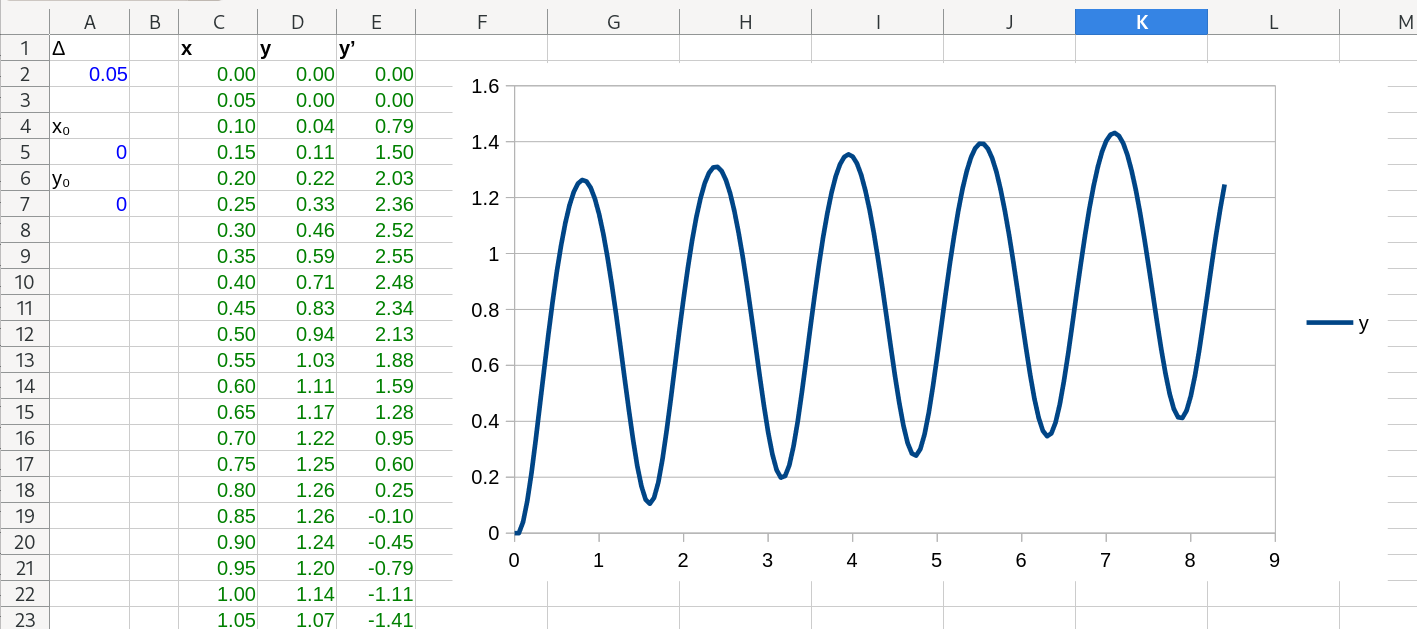
\includegraphics[height=2in]{resources/tutorial-01-sheet1.png}
					\end{center}
					
					Analytically, if $y(x)=0$, then $y'(x) = 0$ for all $x$. However, the differential equation is not the constant zero function.
					
					\item Simulating, we see that the simulated values of $y$ with $\Delta=0.7854$ are extremely tiny.
					\begin{center}
						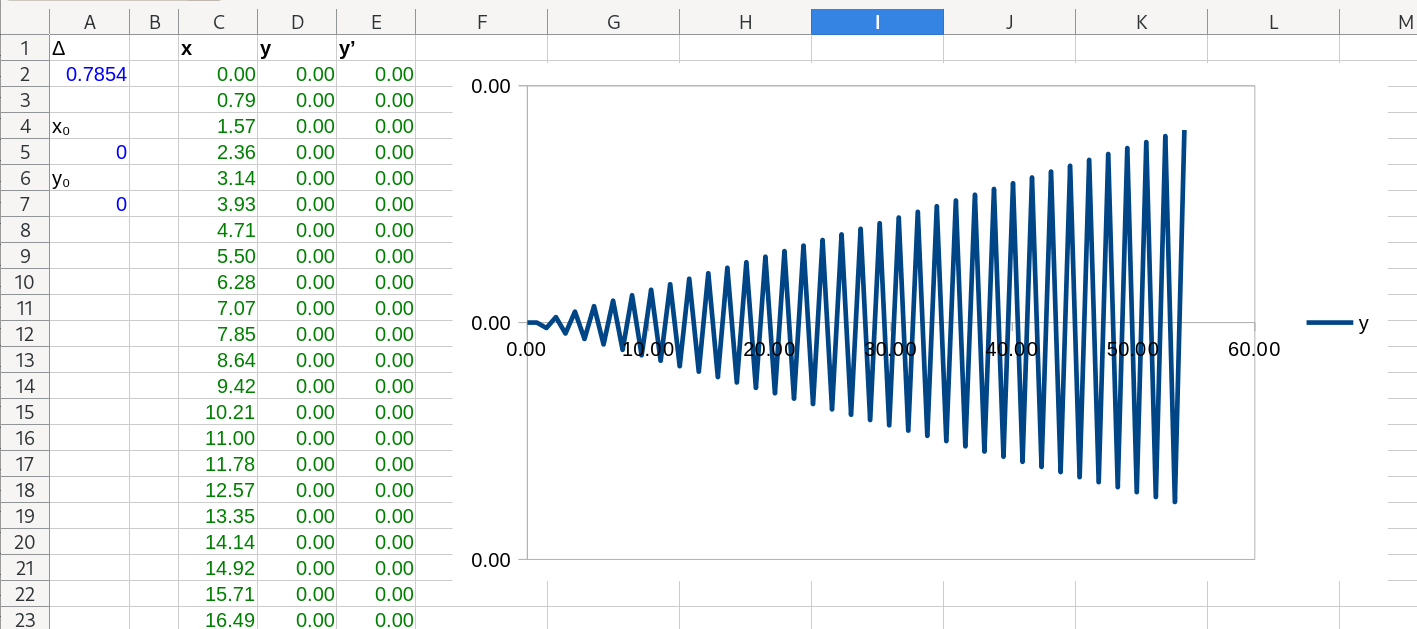
\includegraphics[height=2in]{resources/tutorial-01-sheet1b.png}
					\end{center}
					We know from simulating with other values of $\Delta$ that the values of $y$ do not stay close to zero, so using $\Delta=0.7854$ does
					not lead to a reasonable approximation.
					
					\item Simulating with $\Delta=0.1$, we can look at the data of our spreadsheet to find the local maxima.
					\begin{center}
						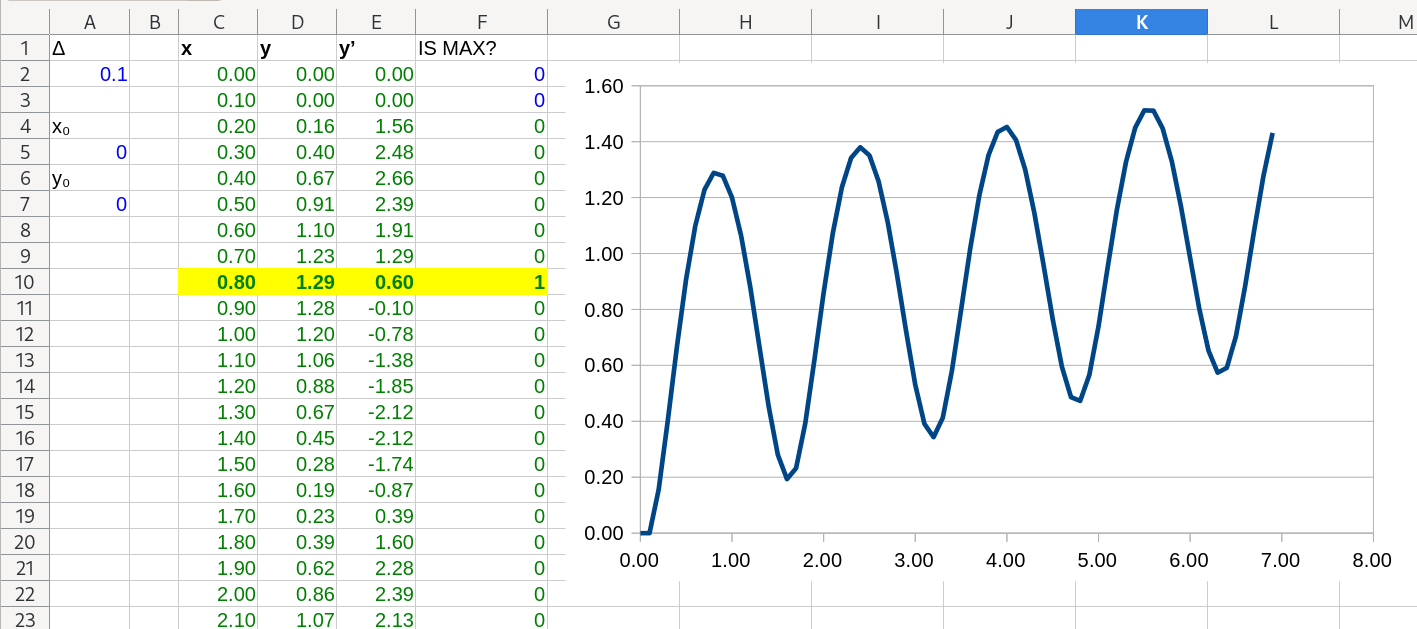
\includegraphics[height=2in]{resources/tutorial-01-sheet1c.png}
					\end{center}
					They occur at $x=0.8, 2.4, 4.0, 5.5,\ldots$.

					\item Local maxima occur when $y'=0$ and $y''\leq 0$ (note when $y''=0$, further testing is required).
					From the differential equation, we can see that $y'(x)=0$ when $x$ is a multiple of $\frac{\pi}{4}$.
					Computing the second derivative,
					\[
						y''(x) = \frac{16\cos(4x)}{1+y} - \frac{4\sin(4x)}{(1+y)^2}.
					\]
					Testing $y''$ when $x=n\frac{\pi}{4}$, we see that it is negative when $n=2k+1$, so we have local maximums at
					$x=\pi/4, 5\pi/4, 9\pi/4, 13\pi/4,\ldots\approx0.79,2.36,3.92,5.50,\ldots$, which is close to our numeric approximations
					from the previous part.

			\end{enumerate}
			\item \begin{enumerate}
					\item Making a table of values, we have

					\begin{tabular}{l|l|l|l|l}
						$\Delta$&Max 1&Max 2&Max 3 &Max 4\\
						\hline
						$0.1$    & 1.29 & 1.38 & 1.45 & 1.51 \\
						$0.05$   & 1.26 & 1.31 & 1.35 & 1.39 \\
						$0.01$   & 1.24 & 1.25 & 1.26 & 1.27 \\
						$0.005$  & 1.24 & 1.24 & 1.25 & 1.25
					\end{tabular}

					\item Numerical evidence suggests that the solutions are periodic without an upward drift. As $\Delta$ is
					made smaller and smaller, the difference in height between the first four peaks gets smaller and smaller and
					seems to converge $\sim 1.24$. Since we already know that the local maxima appear at regular intervals, this suggests
					that the peaks are not drifting and the solution as a whole is periodic.

					\item Computing, $\displaystyle A'(x) = \frac{4\sin(4x)}{\sqrt{3-2\cos(4x)}} = \frac{4\sin(4x)}{A(x)+1}$, which fits the form
					of the differential equation.

					\item $A$ is a periodic solution to the differential equation satisfying $A(0)=0$, so there must be a periodic solution to
					the differential equation.
			\end{enumerate}
			\item \begin{enumerate}
				\item Modifying the previous spreadsheet we get
					\begin{center}
						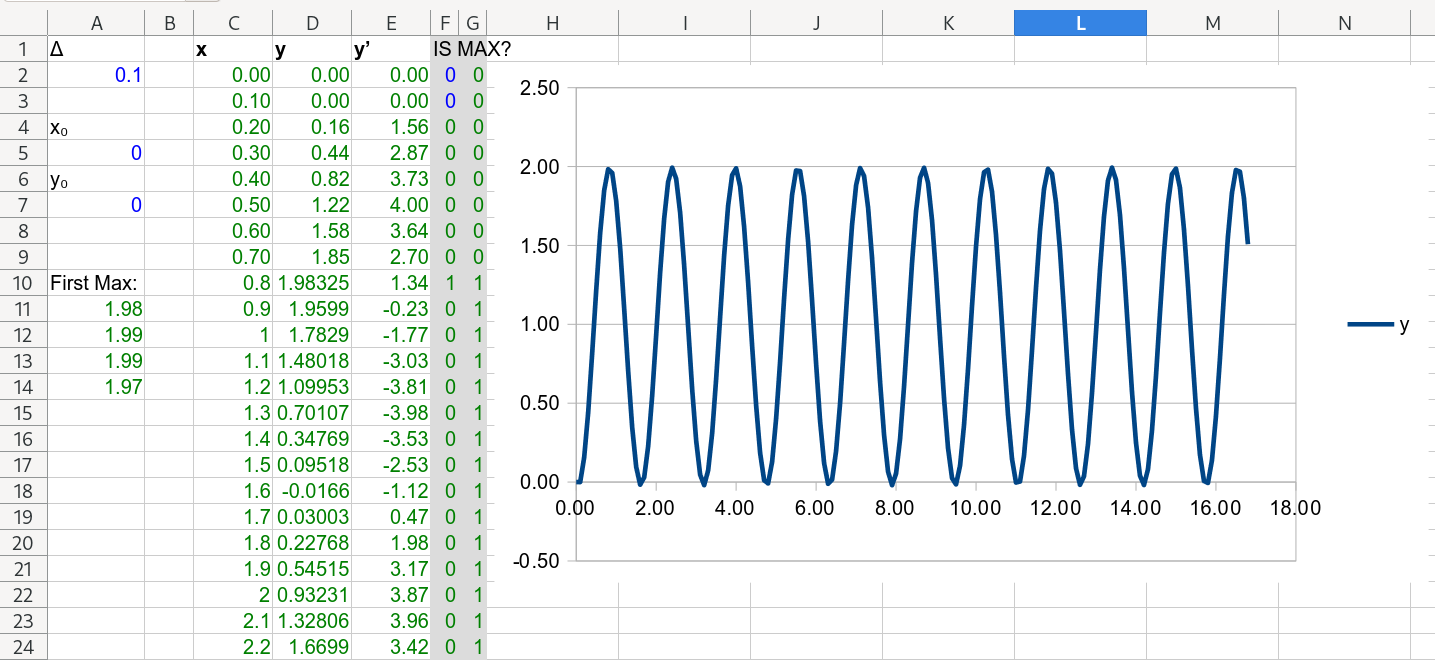
\includegraphics[height=2in]{resources/tutorial-01-sheet3a.png}
					\end{center}
				\item An exect solution satisfying $y(0)=0$ (found by integration) is $y(x)=-\cos(4x)+1$.
					Plotting, we see that the error doesn't increase much compared to $x$.
					\begin{center}
						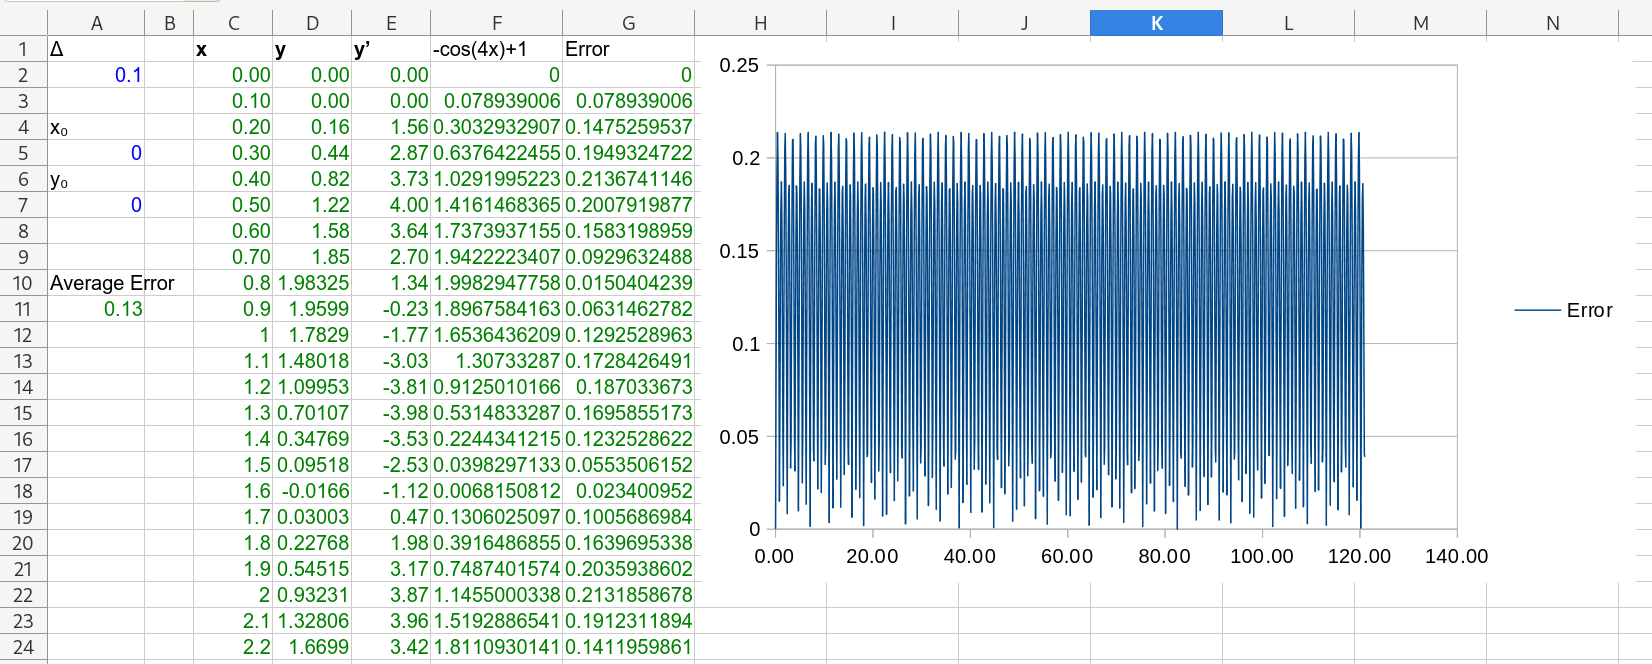
\includegraphics[height=2in]{resources/tutorial-01-sheet3b.png}
					\end{center}
				\item We have seen two cases of Euler's method producing errors. For the first differential equation, errors did accumulate, but in the second
					differential equation, errors did not end up accumulating. The conclusion is, you cannot always assume that errors end up
					accumulating when using Euler's method (you must do an analysis on a case-by-case basis)!

			\end{enumerate}
		\end{enumerate}

	
	\end{solutions}
	\begin{instructions}
				\subsection*{Learning Objectives} Students need to be able to\ldots
		\begin{itemize}
			\item Explore how different parameters affect the qualitative
				behaviour of solutions to a system of differential equations.
			\item Translate back and forth between a model's equations and
				the real-world situation that the model describes.
		\end{itemize}


		\subsection*{Context} In class we have studied the Fox and Rabbit
		Lotka-Volterra system with fixed parameters. We have made a phase portrait
		and simulated solutions using multi-dimensional Euler's method with
		a spreadsheet. We also analyzed equilibrium solutions and their
		relationship to phase portraits. However, we have only done this once.
		Students need more practice!


		\subsection*{What to Do} This is the first tutorial of the term, and
		it is your chance to win the students over! This is a groupwork tutorial,
		but students may not be used to working in groups.

		\begin{itemize}
			\item Arranged for group work. Reorganize the desks and chairs
				(if possible) to facilitate groups of 3 or 4. Ask
				students to form groups of 3 or 4 with other students
				nearby. Don't allow larger groups.

			\item Begin the tutorial by introducing yourself (your name,
				your program of study, and your year). You might
				also want to give them some more personal information,
				such as where you are from or when you first started liking math.

			\item Introduce the structure and purpose of tutorials: students
				will be working to (1) better understand concepts
				from lecture, (2) practice tackling concepts that
				have not been explained in lecture, and (3) effectively
				communicate. They can expect to spend most of the
				tutorial working in small groups.

			\item Emphasize the importance of working with others when
				learning mathematics---they should be working with
				others in this tutorial \emph{and} outside of
				class.
		\end{itemize}

		This introduction should take no more than 5 minutes.

		Next, introduce the learning objectives for the day's tutorial. Explain
		that the goal of this tutorial. Their worksheet has the ``formal'' objectives
		stated and these instructions have the ``hidden'' objectives. Feel free
		to share with them the hidden objectives as well.

		Ask the students to pair up and
		start working on the problem list. Circulate around the room during
		this time and ask groups what they're thinking. They will be tempted
		to move quickly through the list without thoroughly checking their
		new answers---encourage them to think deeply.

		Problem 1 is a straightforward question, but students will struggle starting
		with part (d) and especially with (e) and (f). They may have forgotten about unions! Ask
		them to review the set operations that they know and be creative. When most people are on
		parts (e) and (f), go over parts (a)--(d). Then, let them continue working through number 2.
		If most of the class gets stuck at any point, draw the class's attention to the front
		of the room and work on the difficult part together.

		There are too many problems to finish in 50 minutes and \emph{you should not be going
		over the solution to every problem}. Solutions will be posted for the students. The goal
		of tutorial is for students to spend time \emph{doing} mathematics with an expert around
		to help them if they get stuck. Don't feel any time pressure, even if you only get through 1.5
		questions, that's okay!

		During the last 6 minutes of class, pick one problem (perhaps a few parts of one problem)
		that most groups have at least started, and do this problem as a wrapup. Seeing an expert do the
		problem is the student's reward for working so hard.

		Notes:
		\begin{itemize}
			\item Students won't have a good conceptualization of convex combinations which make 1(f) and 3(c).
				These problems can also be done by describing a line in vector form (i.e., $\vec x=t\vec d+\vec p$)
				and restricting the scalar to get points on the line segment.
			\item For 1(e), some students might write $\{\vec x:\vec x\text{ is a convex linear combination
				of }\vec p\text{ and }\vec q\}$. Other students might think that this description
				is ``mathy'' enough. This description is mathy enough, but we can also expand it
				by inserting the definition of \emph{convex linear combination} into the set.
			\item Problem 2 is more open-ended than they're used to. Some will get excited about this, and others will
				be turned off because it's not a ``plug and chug'' question. Emphasize to them that
				they will be hired for their creativity and problem-solving, and not their ability to
				answer precisely laid out questions, and this is what we're practicing!
			\item Students will be confused what part 2(d) means. If so, take some time at the front of the room
				to make a chalk drawing of a face and a reverse face.
				Remember, if you're writing on a chalkboard, black and white are already reversed!
		\end{itemize}

	\end{instructions}

\end{document}
